\documentclass{article}

\usepackage{hyperref}
\usepackage{geometry}
\usepackage{changepage}
\usepackage{graphicx}
\usepackage[export]{adjustbox}
\usepackage{titlesec}
\usepackage{xcolor}
\hypersetup{
    colorlinks,
    linkcolor={red!50!black},
    citecolor={blue!50!black},
    urlcolor={blue!80!black}
}

\setlength\parindent{0pt} % noindet
\setcounter{secnumdepth}{4}

\geometry{legalpaper, margin=1in}

\graphicspath{{../img/}}

\titleformat{\paragraph}
{\normalfont\normalsize\bfseries}{\theparagraph}{1em}{}
\titlespacing*{\paragraph}
{0pt}{3.25ex plus 1ex minus .2ex}{1.5ex plus .2ex}

\begin{document}

\large{\textbf{Dr Thomas Huet}}\\
%\begin{itemize}
\normalsize
EAMENA Researcher and Database Manager\\
\small
Endangered Archaeology in the Middle East and North Africa\\
\normalsize
University of Oxford, School of Archaeology\\
\small
2 South Parks Road, Oxford OX1 3TG, United Kingdom
\normalsize
%\end{itemize}
\\
\smash{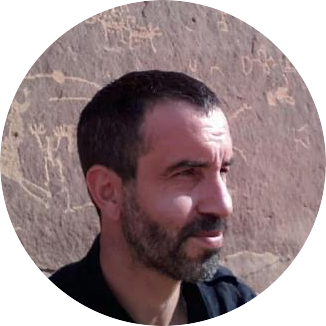
\includegraphics[width=3.5cm, right]{id-r}}

\includegraphics[scale=0.025]{gmail} \quad \href{mailto:thomas.huet@arch.ox.ac.uk}{thomas.huet@arch.ox.ac.uk} \& \href{mailto:thomashuet7@gmail.com}{thomashuet7@gmail.com}\\

\includegraphics[scale=0.01]{webpro} \quad \href{https://archit.web.ox.ac.uk/people/dr-thomas-huet}{School of Archaeology} \& \href{https://eamena.org/people/dr-thomas-huet}{EAMENA project}\\

\includegraphics[scale=0.007]{orcid} \quad \href{https://orcid.org/0000-0002-1112-6122}{0000-0002-1112-6122} \\

\includegraphics[scale=0.007]{github} \quad \href{https://github.com/zoometh/thomashuet.github.io/blob/main/README.md}{zoometh} \\

\includegraphics[scale=0.025]{gscholar} \quad \href{https://scholar.google.fr/citations?user=2hKEVaIAAAAJ}{2hKEVaIAAAAJ} \\

\includegraphics[scale=0.05]{rgate} \quad \href{https://www.researchgate.net/profile/Thomas\_Huet2}{Thomas\_Huet2} \\

\includegraphics[scale=0.005]{phone} \quad  \+ 44 (0)7 518 152 642 \\

\\

\begin{adjustwidth}{50pt}{50pt}
\begin{center}
\large{\textbf{Curriculum Vitae}}\\
\large{Prehistory, Cultural Heritage \& Computational Archaeology} 
\end{center}
\end{adjustwidth}

\section{ACADEMIC \textit{\&} PROFESSIONAL POSITIONS (2014-)}

\textbf{since 2021 }EAMENA Researcher and Database Manager, University of Oxford, School of Archaeology, 2 South Parks Road, Oxford OX1 3TG, United Kingdom, 1 November-...
\smallbreak
\textbf{--- }Specialist Research Support Technician, Departament de Prehist\`oria, Universitat Aut\'{o}noma de Barcelona (UAB), Spain, 1 July-31 December.
\smallbreak
\textbf{2020 }Co-responsible of the survey of the medieval engravings of Sauri (Catalonia, Spain), 2${}^{nd\ }$campaign, Universitat Aut\'{o}noma de Barcelona (UAB), Spain, 19 October-24 October.
\smallbreak
\textbf{2019-20 }Researcher at Archa\"{i}os company, in charge of the database integration for the survey of Al-'Ula, Saudi-Arabia (Archa\"{i}os, AFALULA, RCU).
\smallbreak
\textbf{2019 }Co-responsible of the survey of the medieval engravings of Sauri (Catalonia, Spain), 1${}^{st\ }$campaign, Universitat Aut\'{o}noma de Barcelona (UAB), Spain, 15 September-15 October.
\smallbreak
\textbf{--- }Project designer for the creation of a technological hub in Emerging technologies for Humanities, UMR 8546 CNRS/PSL-AOrOc, Paris, resp. K. Gruel. 1 June-1 July.
\smallbreak
\textbf{2018 }Research Engineer (IR), UMR 7264 CEPAM---CNRS, Universit\'{e} Nice Sophia-Antipolis, project \textit{C\'{e}ramiques Imprim\'{e}es de M\'{e}diterran\'{e}e occidentale} (CIMO), resp. D. Binder, 1 May-30 August, and 1 October-30 November.
\smallbreak
\textbf{--- }Research Engineer (IR), UMR 5140, ASM-CNRS, Universit\'{e} Paul Val\'{e}ry Montpellier 3, project \textit{EpiSpat} (aka \textit{ArchaEpigraph}), LabEx ARCHIMEDE, resp. C. Pellecuer, 1 April-1 May, and 1-30 September.
\smallbreak
\dots
\smallbreak
\textbf{2006-12 }PhD History and Archaeology, title: 'Organisation spatiale et s\'{e}riation des gravures piquet\'{e}es du mont Bego', first level of distinction (mention tr\'{e}s honorable avec les f\'{e}licitations du jury), 29 May 2012, Universit\'{e} Nice Sophia-Antipolis, UMR 7264 CEPAM-CNRS, HALtheses: \href{https://tel.archives-ouvertes.fr/tel-00712290}{tel-00712290}.
\smallbreak

\section{SELECTED PUBLICATIONS (2014-)}
**: book, *: book chapter, \textsuperscript{1}: research article
\smallbreak
$\cdot$ \textbf{Huet T., 2017}, \textit{Les gravures piquet\'{e}es du mont Bego (Alpes-Maritimes). Organisation spatiale et s\'{e}riation (6e -- 2e mill\'{e}naire av. J.-C.)}, M\'{e}moire de la Soci\'{e}t\'{e} Pr\'{e}historique Fran\c{c}aise (SPF) 63, 166 p. \href{http://www.prehistoire.org/shop_515-40342-0-0/m63-2017-les-gravures-piquetees-du-mont-bego-alpes-maritimes-organisation-spatiale-et-seriation-vie-iie-millenaire-av.-j.-c.-t.-huet.html}{
\includegraphics[scale=0.02]{link_darkblue.png}}.**
\smallbreak
$\cdot$ Alexander C., Maretta A., \textbf{Huet T.} and C. Chippindale, \textbf{2021}, Rules of ordering and grouping in the 'pitoti', the later prehistoric rock-engravings of Valcamonica (BS), Italy: from solitary figures through clusters, graphic groups, and scenes to narrative, in I. Davidson and A. Nowell (eds), \textit{Making scenes: global perspectives on scenes in rock art}, London: Berghahn Books, p. 259-276 \href{https://www.berghahnbooks.com/title/DavidsonMaking}{
\includegraphics[scale=0.02]{link_darkblue.png}}.*
\smallbreak
$\cdot$ \textbf{Huet T., 2018}, Une revue de l'iconographie du d\'{e}but du N\'{e}olithique \`{a} la fin de l'\^{a}ge du Bronze (ca. 5700-750 av. J.-C.) en France, \textit{in} Guilaine J. et D. Garcia (dir.), \textit{La Protohistoire de la France}, ed. Hermann, Paris, p. 221-249, HAL: \href{https://hal.archives-ouvertes.fr/hal-01983284}{hal-01983284}.*
\smallbreak
$\cdot$ Binder D., Gomart L., \textbf{Huet T.}, Ka{\v{c}}ar S., Maggi R., Manen C., Radi G., Tozzi C., with the collaboration of Mutoni I.M., Natali E. and C. Panelli, \textbf{to be published}, Le complexe de la C\'{e}ramique imprim\'{e}e de M\'{e}diterran\'{e}e centrale et occidentale : une synthèse chrono-culturelle (7e et 6e millénaires BCE), in Binder D. and C. Manen (dir), \textit{C\'{e}ramiques imprim\'{e}es de M\'{e}diterran\'{e}e occidentale (6e mill\'{e}naire BCE) : Donn\'{e}es, approches et enjeux nouveaux. Actes des journ\'{e}es de la Soci\'{e}t\'{e} Pr\'{e}historique Fran\c{c}aise, Nice, 18-20 mars 2019}, Paris: Soci\'{e}t\'{e} Pr\'{e}historique Fran\c{c}aise.\textsuperscript{1}
\smallbreak
$\cdot$ \textbf{Huet T.}, Cubas M., Gibaja J.F., Oms F.X. and Mazzucco N., \textbf{2022}, NeoNet Dataset. Radiocarbon Dates for the Late Mesolithic/Early Neolithic Transition in the North Central-Western Mediterranean Basin, \textit{Journal of Open Archaeology Data}, DOI: \href{http://doi.org/10.5334/joad.87}{10.5334/joad.87}.\textsuperscript{1}
\smallbreak
$\cdot$ \textbf{Huet T.}, Pozo J. M., Alexander C., \textbf{2021}, Analysis of Prehistoric Iconography with the R package \textit{iconr}, \textit{Journal of Open Statistical Software}, \href{https://joss.theoj.org/papers/10.21105/joss.03191}{10.21105/joss.03191}.\textsuperscript{1}
\smallbreak
$\cdot$ Nieto-Espinet A., \textbf{Huet T.}, Trentacoste A., Guimaraes S., Orengo H. and Valenzuela-Lamas S., \textbf{2021}, Resilience and livestock adaptations to demographic growth and technological change: A diachronic perspective from the Late Bronze Age to Late Antiquity in NE Iberia, \textit{PlosONE}, DOI: \href{https://doi.org/10.1371/journal.pone.0246201}{10.1371/journal.pone.0246201}.\textsuperscript{1}
\smallbreak
$\cdot$ Iba\~{n}ez J.J., Mu\~{n}iz J., \textbf{Huet T.}, Borrell Terra F.,.Santana Y., Teira Mayolini L.C. and R. Rosillo, \textbf{2020}, Flint Figurines in the Early Neolithic site of Kharaysin (Early 8th Millennium BC, Jordan), \textit{Antiquity Journal, 94, 376} p. 880-899, DOI: \href{https://doi.org/10.15184/aqy.2020.78}{10.15184/aqy.2020.78}.\textsuperscript{1}
\smallbreak
$\cdot$ Cicolani V. and \textbf{T. Huet, 2019}, Essai de mod\'{e}lisation des \'{e}changes et des r\'{e}seaux de circulation dans les Alpes centrales au premier \^{a}ge du Fer, \textit{in} "La conqu\^{e}te de la montagne : des premi\'{e}res occupations humaines \`{a} l'anthropisation du milieu", \textit{Comit\'{e} des Travaux Historiques et Scientifiques \'{e}ditions} (CTHS), DOI: 10.4000/books.cths.7827, HAL: \href{https://halshs.archives-ouvertes.fr/halshs-02314978/document}{halshs-02314978}.\textsuperscript{1}
\smallbreak
$\cdot$ \textbf{Huet T., 2016}, New perspectives on the chronology and the meaning of Mont Bego's rock-art (Alpes-Maritimes, France), \textit{Cambridge Archaeological Journal} 41, 1-23, DOI: \href{https://doi.org/10.1017/s0959774316000524}{10.1017/s0959774316000524}.\textsuperscript{1}
\smallbreak
$\cdot$ \textbf{Huet T.} and N. Bianchi, \textbf{2016}, A study of the Roche de l'Autel's pecked engravings, Les Merveilles sector, Mont Bego area (Alpes-Maritimes, France), \textit{Journal of Archaeological Sciences: Reports} 5, 105-118, DOI: \href{https://doi.org/10.1016/j.jasrep.2015.11.006}{10.1016/j.jasrep.2015.11.006}.\textsuperscript{1}
\smallbreak

\subsection*{Scientific Conferences Organisation}
\begin{center}(\textbf{i}) \textbf{i}nternational audience {\textbar} (\textbf{n}) \textbf{n}ational audience \end{center}
\smallbreak
\textbf{2022 }CAA2022, Session n$\mathrm{{}^\circ}$ 07: \textit{"Cultural Heritage data across borders. Web-based management platforms for immovable cultural heritage in the global south"}, co-organised with C. El Safadi, B. Rouhani, A. Smith, International congress of the \textit{Computer Applications and Quantitative Methods in Archaeology}, University of Oxford, UK, 8-11 August (\textbf{i})
\smallbreak
\textbf{2022 }9${}^{th}$ Seminar of Technology Prehistoric:\textit{" Confocal microscopy for the analysis of wear on tools and teeth in Prehistory"}, co-organised with Fiona Pichon, Juan Jose Ibanez, Hala Arashi, Hermine Xhauflair, Ferran Estebaranz Sanchez, Laura Martinez, Niccolo Mazzucco, Andrea Zupancich, Sergio Jimenez Manchon, 2-4 May, Institute Milá y Fontanals (CSIC), Barcelona, Spain (\textbf{i})
\smallbreak
\textbf{2016 }S\'{e}minaire d'\'{e}quipe ASM-CNRS (UMR 5140), \'{e}quipe Soci\'{e}t\'{e}s de la Pr\'{e}histoire et de la Protohistoire, Analyser et interpr\'{e}ter les d\'{e}cors des c\'{e}ramiques pr\'{e}- et protohistoriques. Approches crois\'{e}es, co-organised with T. Lachenal et K. Peche-Quichilini, Universit\'{e} Paul-Val\'{e}ry, Montpellier, 27 May (\textbf{n})
\smallbreak
\textbf{2014 }CAA2014, Session n$\mathrm{{}^\circ}$ 20: \textit{"(Re)building past networks: archaeological science, GIS and network analysis"}, co-organised with C. Alexander, S. Robert, E. Mermet, 42${}^{nd}$ international congress of the \textit{Computer Applications and Quantitative Methods in Archaeology}, Universit\'{e} Sorbonne, France, 22-25 April (\textbf{i})
\bigbreak

\section{SELECTED ACADEMIC TEACHINGS \textit{\&} RESEARCH PROGRAMS (2014-)}

\textbf{2022 }"Visiting Fellow", \textit{Dipartimento di Civilt\'{a} e forme del Sapere}, Universit\'{a} di Pisa, 11 March-15 April (1 month).
\smallbreak
\textbf{--- }"Report with R Markdown", Winter School 'R 4 Archeologists', \textit{Progetto metodologie applicate all predittivita del potenziale archeologico} (mappa), Universit\'{a} di Pisa, 4 February (3 hours), \href{https://github.com/zoometh/thomashuet/tree/main/profiles/oxford/R4A#readme}{
\includegraphics[scale=0.12]{github-rect.png}}.
\smallbreak 
\textbf{2017 }"Introduction to Geographic Information Systems: QGIS", \textit{Grupo de Arqueologia de las Din\'{a}micas Sociales}, Consejo Superior de Investigaciones Cientificas, Instituci\'{o}n Mil\'{a} i Fontanals (CSIC-IMF), 14-16 December (9 hours).
\smallbreak
\textbf{2015-... }Member of Francis Bordas PhD steering committee, Universit\'{e} Toulouse 2, \'{E}cole doctorale TESC, UMR TRACES, PhD title: "Les d\'{e}p\^{o}ts d'objets m\'{e}talliques au Bronze final 3 dans l'espace atlantique fran\c{c}ais (950-800 av J.-C.) : modalit\'{e}s de constitution des d\'{e}p\^{o}ts fran\c{c}ais de l'\'{e}tape de l'\'{e}p\'{e}e du type en langue de carpe".
\smallbreak
\textbf{2018-9 }Tutor of Marco Padovan Master 2 steering committee, Universit\'{a} degli Studi di Ferrara, Corso di Laurea Magistrale in Quaternario, Preistoria e Archeologia, "Fabric analysis of the Mesolithic layers at Baume du Monthiver (Comps-sur-Artuby, Var, France)".

\subsection*{Selected Research Programs}

\subsubsection*{Scientific journal committees}

- Member of the editorial board of the \textit{Pr\'{e}histoires M\'{e}diterran\'{e}ennes} journal (2021-...)\\ 
- Reviewer for the \textit{ArcheoLogica-Data} journal (2022-...)\\
- Reviewer for the \textit{Journal of Open Source Software} (2021-...)\\
- Reviewer for the \textit{Bulletin de la Soci\'{e}t\'{e} Pr\'{e}historique Fran\c{c}aise} journal (2020-...)\\
- Reviewer for the \textit{CAA Review College} (2014-...)\\ 

\subsubsection*{Collective research projects}

- Member of the \href{https://sslarch.github.io/}{SIG-SSLA} Special Interest Group on Scientific Scripting Languages in Archaeology.(2020-...)\\ 
- Member of the \href{https://arqueologiademuntanya.wordpress.com/}{GAAM} Grup d'Arqueologia de l'Alta Muntanya (UAB, CSIC) (2020-...)\\ 
- Member of the \href{https://redneonet.com/}{NeoNet} collective research project, resp. J. Gibaja, M. Cubas (2020-...)\\ 

\end{document}
